\chapter[Chapter 3: Research Methodology]{Research Methodology}

\section{Background}

We will use a mixed method study in order to gain a complete understanding of the \gls{cita} on \gls{chip} system. Quantitative analysis will be used to find trends in student grades between classes that do and do not use the program. In parallel, we will conduct a qualitative study to determine student reactions to the program and how they feel their learning was affected. A breakdown of our methodology is shown in Figure \ref{fig:flowchart}.

\begin{figure}[!htb]
	\centering
	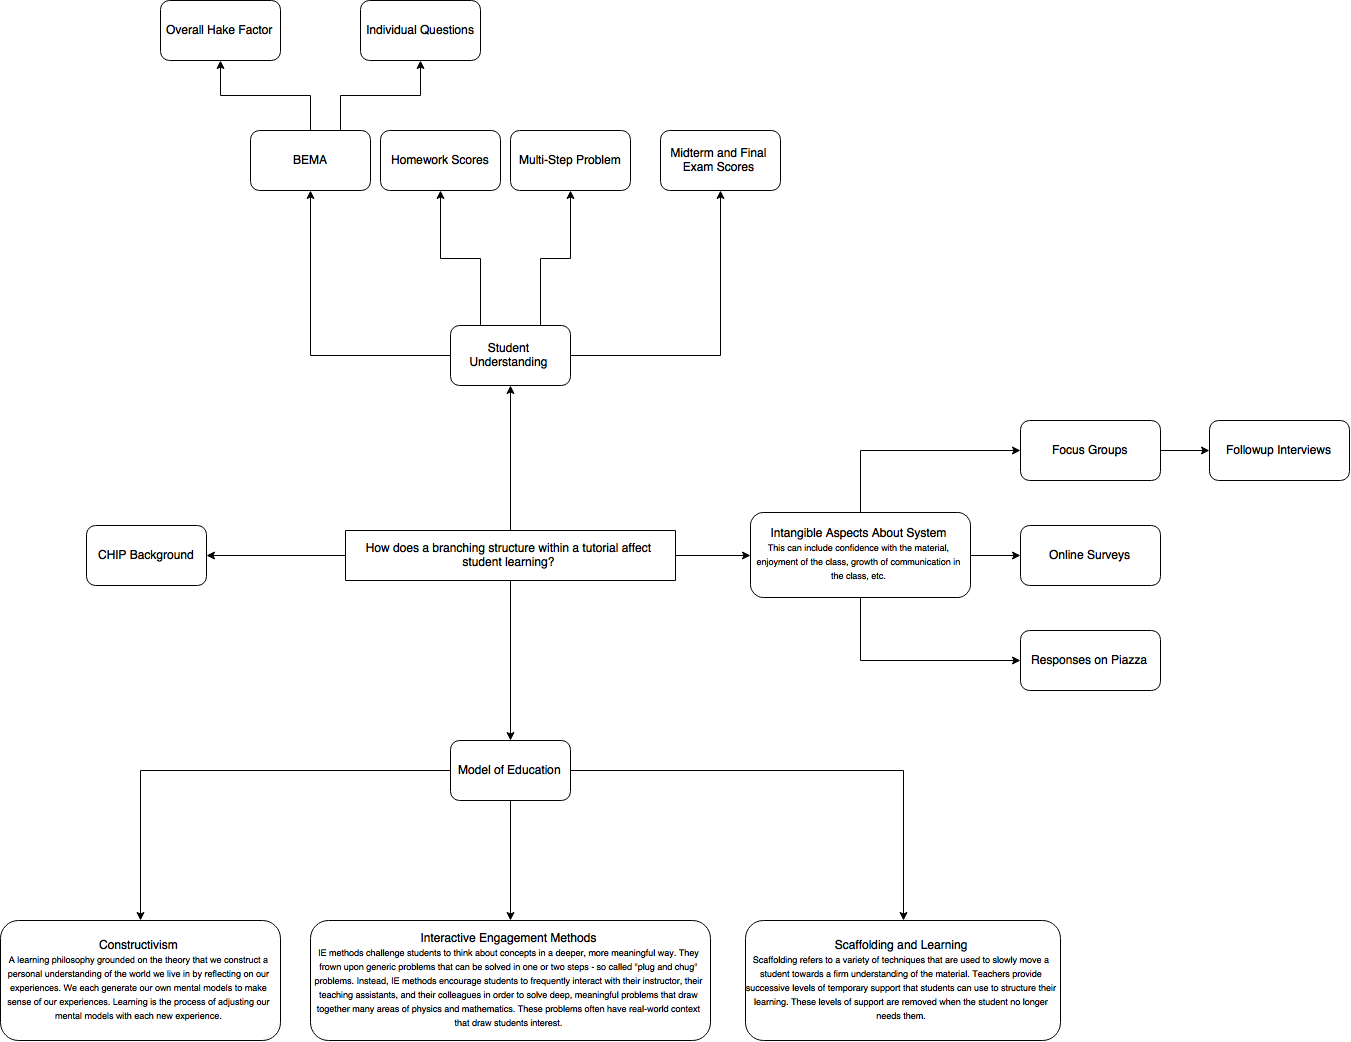
\includegraphics[width=6in]{img/chapter3/flowchart}
	\caption[Flowchart]{Flowchart}
  \label{fig:flowchart}
\end{figure}

\section{Setting and Context}

The population that we are studying is engineering and science students at Purdue University who are taking their second semester of introductory physics. This population contains both domestic and foreign students.

The combined yearly enrollment of PHYS 24100 and PHYS 24100D has an average of about 1500 students from science and engineering. Additionally, we have seen an increase in the number of students in online sections ever since the distance learning course was started in the summer semester of 2012.

\section{Quantitative Inquiry}

\subsection{Grade Data}

Since the \gls{cita} on \gls{chip} program is centered around the homework assignments, we need to analyze how students perform on the homework and how their use of the tutorials influences their other quiz and exam scores. Within \gls{chip}, we can track the level to which students delve into the tutorial. Thus, we can determine who specifically is using \gls{cita} and how often.

Student performance on quiz and exam problems that are similar to \gls{cita} problems will be used to determine if \gls{cita} improved learning outcomes (i.e. whether or not students have learned specific problem solving strategies). We can correlate exam scores with:

\begin{itemize}
\item When students started using \gls{cita} (before or after first exam, first homework, etc.)
\item How many attempts on a problem are made before using \gls{cita}
\item How many attempts to solve a problem are needed after using \gls{cita}
\item After using \gls{cita} on one problem is it used on every problem
\item Comparison of performance on \gls{cita} problems vs. non-\gls{cita} problems
\end{itemize}

\subsection{Brief Electricity and Magnetism Assessment (BEMA)}

Concept inventories and assessment instruments are a useful method of assessing student knowledge of the material; however, they are not simply tests that can be quickly put together and administered year after year. Lindell and Ding describe how it takes years to determine the validity and reliability of the results of a given concept inventory. They describe how reliability (precision) and validity (accuracy) play a role in the inventories and cite how factors such as age, course structure, geography, language, delivery of the tests, and wording of questions can influence the results of the assessment\cite{lindell2012}.

The \gls{bema} was developed by Ruth Chabay, Bruce Sherwood, and Fred Reif in 1997. Although it was originally designed to measure student retention of electricity and magnetism concepts three months to five semesters after completing an introductory electricity and magnetism course, it is now often used to analyze student learning between the beginning and end of the semester. It is a useful tool to assess the understanding of electricity and magnetism concepts that are covered in a college-level calculus-based introductory physics course\cite{ding2006}.

The \gls{bema} is a multiple choice test consisting of qualitative questions and a few simple calculations. Lin Ding et al. performed an analysis of the \gls{bema}, showing that it is a reliable assessment tool for introductory electricity and magnetism courses\cite{ding2006}. We use the \gls{bema} extensively in our research to analyze student's understanding of the course material.

\subsection{Force Concept Inventory}

The \gls{fci}􏰁 is a multiple choice test that is used to measure a student's understanding of introductory mechanics. It is given at the beginning of an introductory mechanics course as a pre-test and again at the end of the course as a post-test. The pool of answers on the test are designed to correspond to common student misconceptions of mechanics; they were developed through a series of student interviews\cite{hestenes1992}. Coletta et al. have observed a strong correlation between the normalized gain on the \gls{fci} and SAT scores. They go so far as to state that SAT scores might be a good indicator of the expected normalized gains within a classroom\cite{coletta2007}.

It is worth mentioning the \gls{fci} here because it is one of the standardized tests used to assess student knowledge of mechanics concepts in PHYS 17200 - the prerequisite to this course. Thus, students should be accostomed to concept inventory exams when they come into PHYS 24100 or PHYS 24100D.

\section{Qualitative Inquiry}

\subsection{Strategy of Inquiry}

We will use focus group sessions to gather information about student's opinions of the \gls{cita} program. One of the many strengths of focus groups is that they are flexible; they can be used for exploratory, explanatory, and evaluative research. Due to this flexibility, focus groups can naturally fit into mixed method research.

Focus groups create a large volume of data with a range of viewpoints. Furthermore, a skilled moderator can ensure that this data has limited researcher influence. In a one-on-one interview, the interviewer cannot help but insert some of his or her own views into the discussion due to the questions asked. However, a focus group can “veer off topic”. Since the group can discuss what they feel is important, they can illuminate important points that the moderator might miss.

Ideally, a focus group should recruit strangers that have knowledge of the material, but no knowledge of each other's opinions. Recruiting total strangers will be somewhat difficult in this study. We will not know if the students in my focus group session have worked together on physics homework beforehand. However, by separating the students in the same section, we should keep the populations reasonably homogeneous, yet randomized.

We would like to divide the pool of student volunteers up into six groups. First, I will separate them if they were in the online or on-campus sections of Electricity and Optics. Then, I will divide them up based on their overall view of the tutorials - generally positive, generally negative, or neutral. Although a student’s opinion on the interactive tutorials would not be considered “highly confrontational”, as Hennink describes, it will be useful to hold separate groups for each viewpoint so as to probe each opinion fully.

I would like to get six people for each group (a total of 36 people per semester). If we cannot collect enough volunteers or if the volunteers are skewed one way or another, we will keep the number in each group the same in order to make sure that there are good discussions. Instead, we will mix the neutral population with the two extremes, being careful to balance each side out.

If students are interested in sharing more information after the focus group session has ended, we will give them the chance to come in for a one-on-one interview. There, we can delve deeper into their own individual thoughts on \gls{cita}.

\subsection{Role of the Researchers}

I have been a teaching assistant for PHYS 24100 and PHYS 24100D since the fall semester in 2011. I have coordinated the course during summer sessions and helped develop the online sections. This includes editing course videos, online recitation format, and online forum. I am currently a senior teaching assistant at Purdue, giving help and advice to other graduate students who are teaching Electricity and Optics.

Professor Hisao Nakanishi has taught PHYS 24100 in the past. More importantly, he is the ``father'' of \gls{chip}. Professor Nakanishi continually makes updates to the content, functionality, and robustness of the \gls{chip} system. He also addresses student questions sent through \gls{chip} about possible errors in the codebase.

Professor Laura Pyrak-Nolte has taught the Electricity and Optics course since 2005 and coordinated the course since the fall 2011 semester. She is the lecturer that is seen and heard in the online lecture videos shown to the PHYS 24100D class.

Professors Lynn Bryan and Andrew Hirsch are not directly related to the Electricity and Optics course. Dr. Hirsch is the interim head of the physics department and Dr. Bryann has a dual appointment in physics and education.

\subsection{Planned Analysis Procedures}

Once we have the transcripts and recordings from focus group sessions and followup personal interviews, we will carefully parse the data to find patterns. First, we will transcribe any recordings so that they are easier to analyze. Then, we will sift through them, looking for key words and phrases that describe how students view the program. Finally, we will synthesize these building blocks into a theory of how introductory physics students at Purdue University view the \gls{cita} program. We will use inductive analysis and creative synthesis as my analysis strategy.

\section{Data Collection Procedures}

It is important to protect student records when doing a study like this. \gls{chip} already uses strong security to protect student records - all students and instructors need to sign into the system using a unique username and password. Additionally, the support staff at Purdue University makes sure that students and instructors are only given permission to access data that is pertinent to them.

We will take additional measures to ensure that all of the data from interviews and focus groups are protected. Whenever we transcribe data, we will identify participants with letters or numbers rather than names (participant A, B, C, etc.). If we do decide to store this data on \gls{chip}, it will be put in a separate, private classroom that only the researchers will be able to access.

Finally, we will only analyze grade data after the semester has ended. This will ensure no conflict of interest between the study and student grades. Interviews might have to take place during the semester due to scheduling. However, as stated above the participants will be anonymized in order to protect their identity.

\section{Timeline and Budget}

The timeline for the development, implementation, and assessment of \gls{cita} on \gls{chip} is shown in Table \ref{tab:timeline}. As of the end of the summer semester in 2015, the project is on schedule.

\pagebreak

\begin{landscape}
\begin{table}[!ht]
  \centering
  \begin{tabular}{|l|l|l|}
    \hline
    \textbf{Semester} & \textbf{CITA Content} & \textbf{Learning Assessment}\\
	\hline
	Spring 2015 & Create Branching Help Button for \gls{chip} & \\
	& Create \gls{cita} Homework Problems & \\
	& Design \gls{gui} for \gls{chip} & \\
	\hline
	Summer 2015 & Create \gls{cita} Homework Problems & Begin Preliminary Work on Muffin\\
	& Beta Test of \gls{cita} Homework Problems &  \\
	\hline
	Fall 2015 & Update \gls{gui} for \gls{chip} & Analyze \gls{cita} Data from Spring 2015 \\
	& Update Assessment Tools on \gls{chip} & Analyze \gls{cita} Data from Summer 2015 \\
	& Expand \gls{cita} Problems & Finalize Muffin \\
	\hline
	Spring 2016 & Expand \gls{cita} Problems & Analyze \gls{cita} Data from Fall 2015 \\
	& Create Interactive Graphics for \gls{cita} & Analyze Class Data from 2012-2014 \\
	\hline
	Summer 2016 & Expand \gls{cita} Problems & Analyze \gls{cita} Data from Spring 2016 \\
	& Expand Interactive Graphics for \gls{cita} & \\
	\hline
	Fall 2016 & Expand \gls{cita} Problems & Analyze \gls{cita} Data from Summer 2016 \\
	& Expand Interactive Graphics for \gls{cita} & \\
	\hline
  \end{tabular}
  \caption{Project Timeline}
  \label{tab:timeline}
\end{table}
\end{landscape}

\pagebreak

This work is funded by a grant through the College of Science at Purdue University. The first part of the grant will last through the year 2015. Then, the grant can be renewed for another year (2016).